% !TeX spellcheck = it_IT

\section{Cos'è lo smart working?}
Il termine \textit{smart working} si riferisce alle nuove modalità lavorative all'interno di un organizzazione, resi possibili dagli avanzamenti tecnologici e resi essenziali dalle pressioni economiche, ambientali e sociali. Questi nuovi approcci non nascono da un'idea rivoluzionaria, ma sono il frutto della graduale evoluzione delle nostre pratiche lavorative che sono diventate sempre più collaborative e libere. \\Alla base vi sono tre concetti fondamentali 
\begin{enumerate}
	\item la revisione della leadership e del rapporto tra manager e dipendente, dal controllo alla fiducia;
	\item il ricorso a tecnologie collaborative in sostituzione ai sistemi di comunicazione rigidi;
	\item la riorganizzazione degli spazi di lavoro che vanno oltre le quattro mura di un ufficio.
\end{enumerate}
\newpage
Il risultato dell'applicazione di questi concetti in contesti aziendali è l'aumento della produttività aziendale in un modus operandi che pone al centro dell'attenzione la persona, unificando gli obbiettivi personali e quelli lavorativi. Questo processo responsabilizza il lavoratore che è consapevole e sente propri gli obbiettivi aziendali e non vede più l'organigramma aziendale come una dura piramide da scalare, bensì si sposta l'attenzione dall'organizzazione, centrale nei vecchi modelli, al singolo, cercando di motivarlo e di aumentare la sua dedizione per le attività che svolge.\\
Diminuendo quindi la distanza tra la vita professionale e quella privata, il dipendente valorizza da sè le attività che svolge e risulta più efficace.
Spesso infatti il termine smart working si utilizza per intendere il telelavoro, alla possibilità di lavorare da casa, alla creazione di spazi per il coworking o a posti di lavoro più flessibili. Sebbene sia corretto, il concetto va molto oltre queste cose e risiede nella ridefinizione del lavoro per come lo intendiamo.\\ All'atto pratico la sua potenza non risiede nel fatto che gli smart workers non hanno orari d'ufficio rigidi o che non importi dove lavorino, ma nella richiesta del datore di lavoro,che vincola il lavoratore unicamente a ottenere i risultati previsti nei tempi stabiliti con il massimo della qualità,. Così facendo il subordinato si sente proprietario del proprio lavoro, autonomo in modalità e tempistiche e viene responsabilizzato, imparando a gestire il suo tempo in modo più intelligente. Il controllo in questo modello lascia spazio alla fiducia nei confronti di un sottoposto. Questa lenta rivoluzione è condotta dai mezzi tecnologici che forniscono più alte possibilità di condivisione fra persone, team e società.\\ \newpage
Lo smart work favorisce quindi la nascita di nuove figure lavorative, come manager moderni che guidano dei gruppi di professionisti e gestendone le risorse, passando così da controllore ad un più costruttivo mentore che lavora sulle individualità della persona, che ne trae vantaggi sia professionalmente che personalmente. \\
L'adozione di questo approccio porterebbe anche vantaggi socio economici come la riduzione dell'inquinamento dovuto agli spostamenti tra le abitazioni e i luoghi di lavoro.  \cite{POL}
\begin{figure}[H]
	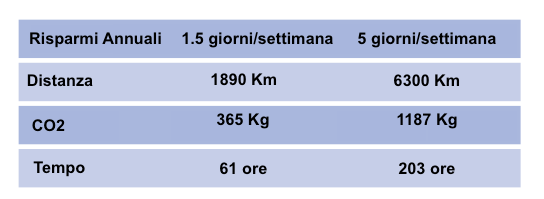
\includegraphics[width=0.35\textwidth]{figure/PolData}
	\centering
		\caption{I dati raccolti da uno studio dell'Università di Oxford sui risparmi ottenuti grazie al telelavoro.}
\end{figure}

\section{I vantaggi del processo di virtualizzazione}
\section{Limiti tecnici}


